\documentclass[border=10pt]{standalone}

\usepackage{tikz}
\usepackage{tikzsymbols}
\usetikzlibrary{calc,patterns,shapes.geometric}

\def\centerarc[#1](#2)(#3:#4:#5){\draw[#1] ($(#2)+({#5*cos(#3)},{#5*sin(#3)})$) arc (#3:#4:#5);}

\begin{document}
	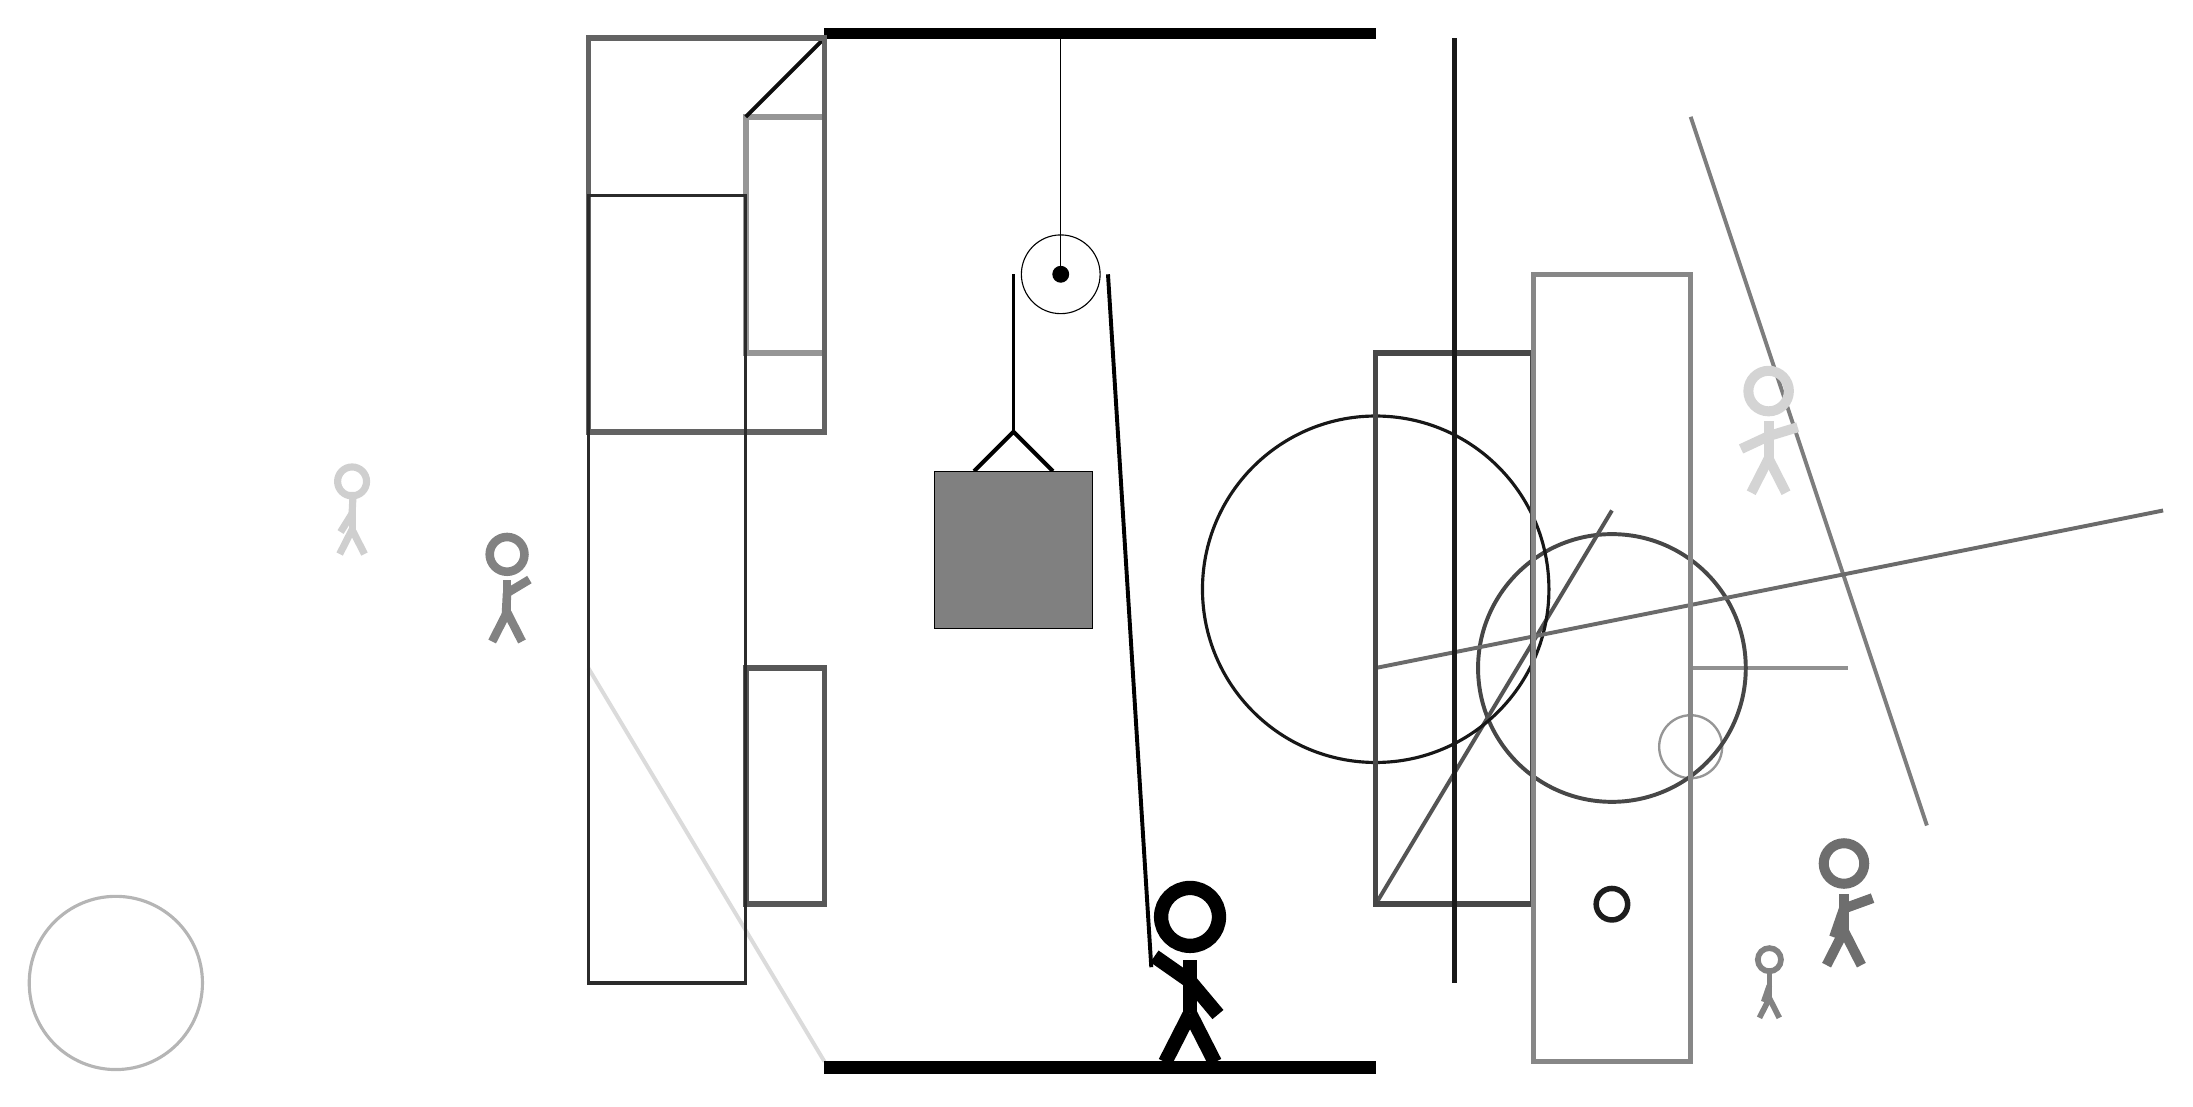
\begin{tikzpicture}
		%%%%% START %%%%%
		
		\draw[fill=black] (-2, 10) rectangle (5, 10.125);
		
		\draw (1, 7) circle (0.5);
		\draw[fill=black] (1, 7) circle (0.1);
		\draw (1, 10) -- (1, 7);
		
		\draw [line width=0.3mm, color=black!41](9, 1) circle (0.4);
		
		\draw [line width=0.7mm, color=black!89](8, -1) circle (0.2);
		\draw [line width=0.4mm, color=black!29](-11, -2) circle (1.1);
		\node[line width=0.5mm, color=black!49] at (10, -2) {\Strichmaxerl[4][71][90]};
		\draw[line width=0.7mm, color=black!41] (-3, 6) rectangle (-2, 9);
		\draw[line width=0.5mm, color=black!51](9, 9) -- (12, 0);
		\draw[line width=0.7mm, color=black!66] (-3, 2) rectangle (-2, -1);
		
		\node[line width=0.4mm, color=black!17] at (10, 5) {\Strichmaxerl[7][25][17]};
		\node[line width=0.5mm, color=black!57] at (11, -1) {\Strichmaxerl[7][71][20]};
		\draw[line width=0.5mm, color=black!43](9, 2) -- (11, 2);
		\draw [line width=0.5mm, color=black!72](8, 2) circle (1.7);
		\draw [line width=0.5mm, color=black!13](-6, 3) circle (0.0);
		\draw[line width=0.5mm, color=black!95](-2, 10) -- (-3, 9);
		\draw[line width=0.5mm, color=black!14](-2, -3) -- (-5, 2);
		\draw[line width=0.5mm, color=black!67](5, -1) -- (8, 4);
		\node[line width=0.4mm, color=black!19] at (-8, 4) {\Strichmaxerl[5][58][87]};
		\draw [line width=0.4mm, color=black!91](5, 3) circle (2.2);
		\node[line width=0.4mm, color=black!49] at (-6, 3) {\Strichmaxerl[6][87][31]};
		\draw[line width=0.7mm, color=black!61] (-2, 5) rectangle (-5, 10);
		\draw[line width=0.5mm, color=black!58](5, 2) -- (15, 4);
		\draw[line width=0.7mm, color=black!72] (5, 6) rectangle (7, -1);
		
		\draw[line width=0.4mm, color=black!83] (-3, 8) rectangle (-5, -2);
		\draw[line width=0.6mm, color=black!90] (6, -2) rectangle (6, 10);
		\draw[line width=0.6mm, color=black!47] (7, -3) rectangle (9, 7);
		
		\draw[line width=0.5mm] (-0.1, 4.5) -- (0.4, 5.0) -- (0.9, 4.5);
		\draw[fill=black!50] (-0.6, 4.5) rectangle (1.4, 2.5);
		
		\draw[line width=0.5mm] (0.4, 7) -- (0.4, 5.0);
		\centerarc[line width=0.5mm](1, 7)(0:180:0.6);
		\draw[line width=0.5mm](1.6, 7) -- (2.15, -1.8);
		
		\node at (2.6, -1.9) {\Strichmaxerl[10][-35][-50]};
		
		\draw[fill=black] (-2, -3) rectangle (5, -3.15);
		
		%%%%% END %%%%%
	\end{tikzpicture}
\end{document}